\chapter{System-level Design}

\section{Testbench Architecture}
The proposed architecture of the verification system shown in Figure \ref{Block}.
The hardware side of this structure is inspired by that of an agent in Universal Verification Methodology (UVM).
Before UVM, integrated circuit designs were verified with methodologies developed independently by simulator vendors such as Cadence, Mentor Graphics, and Synopsys.
In an effort to unify for greater efficiency, the standards organisation of the Electronic Design Automation (EDA) industry, Accellera, established UVM with support from multiple vendors.
It provided a common structure for verification, with class libraries that made building and running a testbench a significantly smoother experience.
The agent is a container in UVM that emulates and verifies DUTs~\cite{Accellera1}.
While this project is in no position to achieve what UVM has done, I do hope that this testbench would have an easily modifiable structure that will make the process of testing similar future designs slightly simpler.

\begin{figure}[H]
  \centering
  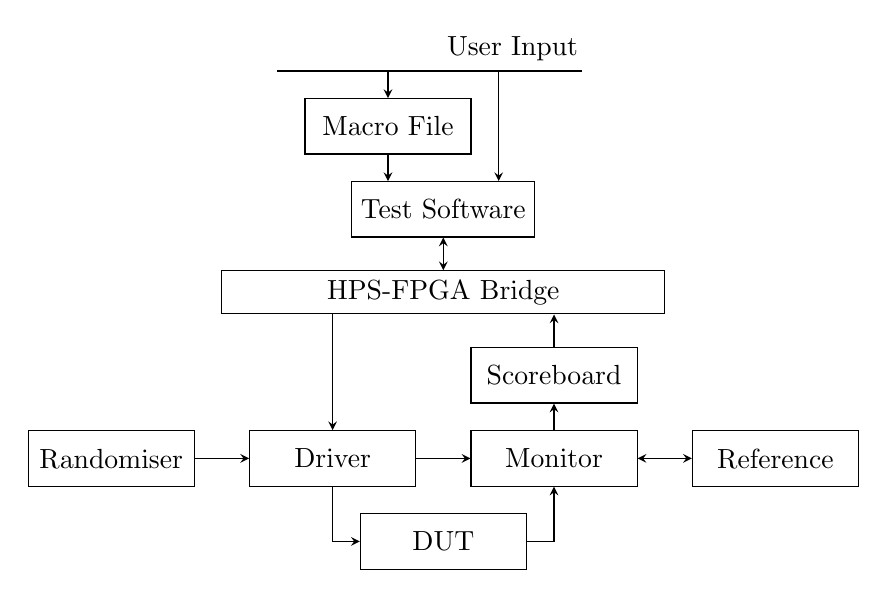
\begin{tikzpicture}
  [
    x=1em, y=1em,
    block/.style =
      {draw, rectangle, align=center, minimum width=6em, minimum height=2em},
    inter/.style =
      {draw, rectangle, align=center, minimum width=16em, minimum height=1em}
  ]
  \node [block] at (-8,3)  (r) {Randomiser};
  \node [block] at ( 0,3)  (d) {Driver};
  \node [block] at ( 4,0)  (t) {DUT};
  \node [block] at ( 8,6)  (s) {Scoreboard};
  \node [block] at ( 8,3)  (m) {Monitor};
  \node [block] at (16,3)  (u) {Reference};
  \node [inter] at ( 4,9)  (b) {HPS-FPGA Bridge};
  \node [block] at ( 4,12) (w) {Test Software};
  \node [block] at ( 2,15) (f) {Macro File};

  \draw[ ->, >=stealth] (r.east)           -- (d.west);
  \draw[ ->, >=stealth] (d.south)          |- (t.west);
  \draw[ ->, >=stealth] (t.east)           -| (m.south);
  \draw[ ->, >=stealth] (m.north)          -- (s.south);
  \draw[ ->, >=stealth] (b.south-|d.north) -- (d.north);
  \draw[ ->, >=stealth] (s.north)          -- (b.south-|s.north);
  \draw[<->, >=stealth] (b.north)          -- (w.south);
  \draw[ ->, >=stealth] (f.south)          -- (w.north-|f.north);
  \draw[ ->, >=stealth] (d.east)           -- (m.west);
  \draw[<->, >=stealth] (m.east)           -- (u.west);
  \draw[ ->, >=stealth] (2, 17)            -- (f.north);
  \draw[ ->, >=stealth] (6, 17)            -- (w.north-|6,17);

  \draw (-2,17) -- ++(6,0) -- node[above] {User Input} ++(5,0);
\end{tikzpicture}
  \caption{Block diagram of the testbench design}
  \label{Block}
\end{figure}

The test software running on the HPS will read instructions from a either a user-written macro file, or straight from the user through command line, and sends the corresponding commands to the hardware.
The driver pulls a stream of random data generated by the randomiser, and converts them to meaningful test inputs according to specification.
The test output will be watched by the monitor, reporting the results to the scoreboard, which keeps track of them.
The monitor make uses of reference designs functionally identical to the DUT, which allows identification of false outputs from the DUT.
Multiple instances of the reference designs means multiple test data can be processed in parallel, so that the reference design can have a relaxed frequency requirement.
The scoreboard collects the results from the monitor and writes them to memory locations accessible from the other side of the bridge.
These memory locations are read by the test scripts, providing results and other useful information to the user.

A major advantage of taking inspiration from the UVM agent structure is its modularity and thus customisability.
Each module has an intuitive purpose and features can be added or removed without much effort.
This fits well with the goal of having an extensible framework.
Since we need at-speed testing capabilities, we have modify the monitor to reference connection to a one to many connection by adding a distributor in the monitor.
Because we also needed precision measurements, the logic of that can be easily added into the scoreboard without affecting other parts of the design.

The design and implementation of each individual hardware and software module will be elaborated in detail in the following chapters.

\section{Hardware Choice}
The system itself will be built on a Cyclone V SX SoC Development Board from Intel~\cite{Intel1}.

\begin{figure}[H]
  \centering
  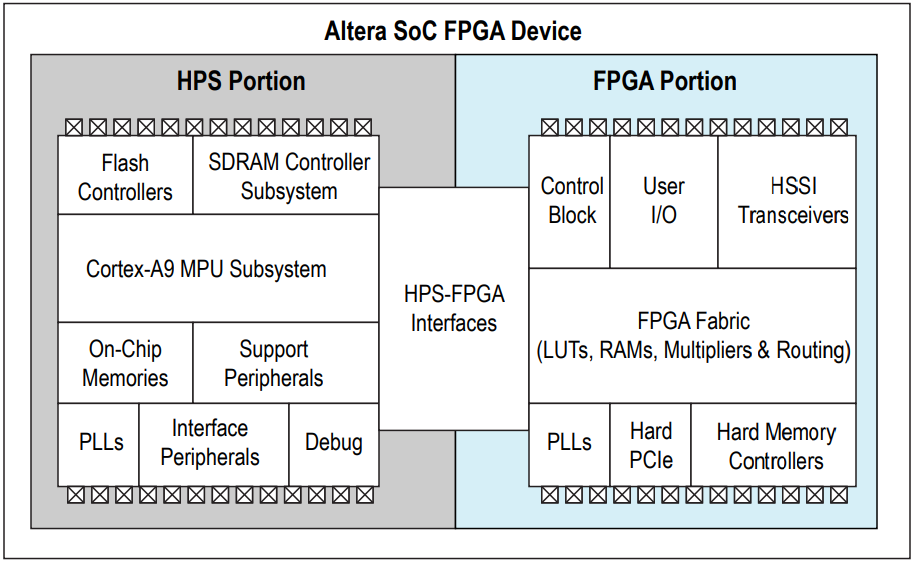
\includegraphics[width=10cm]{img/SoCStructure}
  \caption{Structure of the System-on-Chip}
  \label{SoCStructure}
\end{figure}

The 5CSXFC6D6F31C6N SoC has an Arm Cortex-A9 MPCore accompanied by Intel's 28nm FPGA fabric~\cite{Altera1}.
The FPGA is necessary for implementing the hardware design and obtaining empirical results for the project.
While an FPGA without an embedded CPU would be enough for this project to work, having a Hard Processor System (HPS) on the same chip is useful as the test software can run on it.
The HPS is a separate piece of hardware that distinguishes itself from a soft processor, such as the Nios~II --- a processor programmed onto the FPGA itself.
With this additional capacity, a better user interface can thus be constructed with more detailed, on-the-fly control of the FPGA.
This means setting up the testbench will only require programming the design into the FPGA, followed by running the test script on the HPS.
The product will thus be self-contained.
It will be more accessible as no additional setup is required by the user.

It should be noted that Xilinx offers similar boards as well.
Its Zynq SoC family has a very comparable structure as they too integrate the software programmability of an Arm processor with the hardware possibility of an FPGA.
For example, similar to the Cyclone V SX, Zynq-7000S features an Arm Cortex-A9
coupled with a Xilinx 28nm FPGA~\cite{Xilinx1}.
As such, a board like the ZedBoard~\cite{Xilinx2} could be just as viable for this project.

As there are very few significant functional differences between the two brands, I shall initially explore with the Intel board, simply for its availability and my familiarity with their development tools.
Due to the architectural differences between the logic elements between Xilinx and Altera FPGAs~\cite{Scekic1}, the performances on the two boards are not necessarily identical.
Once the project has progressed to a point where the system design is mature and tested, the Xilinx alternative can be explored as an extension.

\section{Software Choice}
The software choice follows closely with the hardware choice in this project.
To develop for Intel FPGAs, Quartus has to be used.
The version picked is arbitrary as there are not many functional differences between the versions that will be critical to the project.
As Quartus Prime 16.0 is the version installed in the computers in the department, I will use the same version simply for convenience.
This naturally means the hardware system will be built with the system integration tool that comes with Quartus --- Qsys.

The Qsys software is designed to be used for integrating different hardware modules into a system.
As such, it will be used as the interface for the two parallel projects.

In terms the language, we have opted for Verilog for this project.
Since the target DUT will be written in Verilog/VHDL, it makes sense to also use a HDL instead of a HLS language.
The preference of Verilog over VHDL is made simply because I was more familiar with Verilog.

Other than the hardware design tools, there is some freedom of choice on the HPS side of the project.
The test will be built with Python, which will be running on an Ubuntu system that is installed on the HPS.
This choice is made as there are previous unrelated projects on the same development board, which means a lot of time can be saved on tedious setup works such as getting an operating system booting.

Git is used as the version control system for this project.
Two repositories on GitHub holds all files related to this project.

Files related to the implementation of the system are available at:

\indent\indent\url{github.com/MerelyLogical/arithmetic-testbench}

Files related to this report are available at:

\indent\indent\url{github.com/MerelyLogical/final-report}